%--------------------------------------------------------------------
%--------------------------------------------------------------------
% Formato para los talleres del curso de Herramientas Computacionales
% Universidad de los Andes
%--------------------------------------------------------------------
%--------------------------------------------------------------------

\documentclass[11pt,letterpaper]{exam}
\usepackage[utf8]{inputenc}
\usepackage[spanish]{babel}
\usepackage{graphicx}
\usepackage{mdframed}
\usepackage{tabularx}
\usepackage[absolute]{textpos} % Para poner una imagen completa en la portada
\usepackage{multirow}
\mdfdefinestyle{mystyle}{leftmargin=1cm,rightmargin=1cm,linecolor=red}
%\usepackage{pst-barcode}
%\usepackage{auto-pst-pdf}
\usepackage{hyperref}
\decimalpoint


\newcommand{\base}[1]{\underline{\hspace{#1}}}
\boxedpoints
\pointname{ pt}
%\extrawidth{0.75in}
%\extrafootheight{-0.5in}
\extraheadheight{-0.15in}
%\pagestyle{head}

%\noprintanswers
%\printanswers
\renewcommand{\solutiontitle}{}
\SolutionEmphasis{\color{blue}}

\usepackage{upquote,textcomp}
\newcommand\upquote[1]{\textquotesingle#1\textquotesingle} % To fix straight quotes in verbatim

\begin{document}
\begin{center}
{\Large Herramientas Computacionales} \\
Taller 7 - \textsc{Python - Método de Newton-Raphson} \\
{\small \it marzo de 2015}
\end{center}

\begin{textblock*}{40mm}(10mm,20mm)
  
\includegraphics[width=3cm]{logoUniandes.png}
\end{textblock*}

\begin{textblock*}{40mm}(161mm,20mm)
  
\includegraphics[width=3cm]{logoUniandes.png}
\end{textblock*}

\vspace{1cm}

La solución de este taller debe ser presentada en un solo archivo comprimido de nombre \verb+NombreApellido_HW7.tar.gz+, en el cual esté contenido el notebook de iPython con todo el código que solucione la tarea y las dos imágenes: \verb|fractal_lr.png| y \verb|fractal_hr.png|. Para cada punto se dará $1/3$ del puntaje si el código corre, $1/3$ si el código tiene sentido y $1/3$ si el resultado es el apropiado.

\begin{questions}

\question[100] Un fractal es un objeto geométrico que repite su estructura básica a difierentes escalas. Una forma de generar fractales es usando el método de Newton-Raphson para hallar las raíces de una función compleja $f(z)$. Cada punto del plano complejo se colorea en función del resultado de aplicar el método al punto. En este taller vamos a usar la  función $f(z)=z^5+z^2$ y el resultado es el siguiente:

\begin{center}
	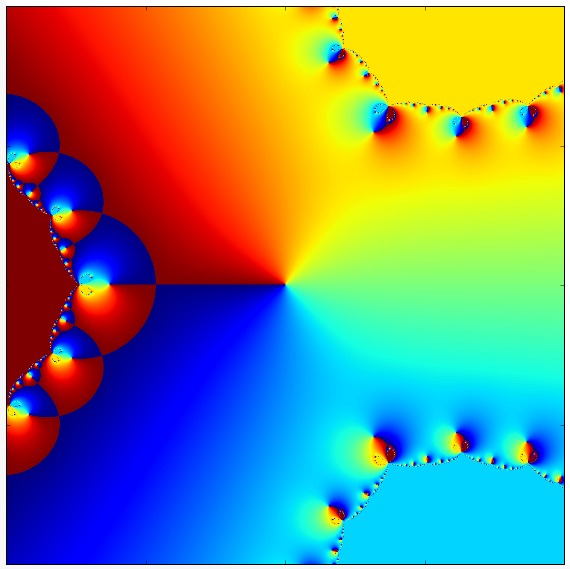
\includegraphics[width=0.85\textwidth]{./fractal_hr.png}
\end{center}

\begin{parts}
\part[20] Escriba dos funciones, una que retorne el valor de la función $z^5+z^2$ y otra que retorne el valor de su derivada.
\part[20] Escriba una función que entregue el resultado de iterar $50$ veces el método de Newton-Raphson para un punto inicial $z$. Esta función debe usar las dos funciones del punto anterior y ser vectorizable. La función debe manejar adecuadamente el problema de la división por cero.
\part[20]\label{latt} Haga un arreglo bidimensional de tamaño $200\times200$, en donde cada elemento del arreglo sea un número complejo  de la región cuadrada del plano complejo que va desde $-1$ a $1$ en la parte real y de $-j$ a $j$ en la parte imaginaria. El elemento $\left[0,0\right]$ de este arreglo debe ser el número complejo $-1+1j$ y el elemento $\left[199,199\right]$ debe ser el número complejo $1-1j$. Esto para que la orientación de los números en el arreglo sean como en el plano complejo usual. Puede usar la función \verb+meshgrid+.
\part[20]\label{proc} Finalmente, aplíquele la función \verb|angle| al arreglo que se generó después de aplicar el método de Newton-Raphson, visualice el resultado con \verb|imshow| y exporte la imagen a un archivo de nombre \verb+fractal_lr.png+ con una resolución adecuada para que el tamaño en pixeles sea de 200 px X 200 px. 
\part[20] Repita los literales \ref{latt} y \ref{proc} pero ahora que sabe que el código funciona, utilice un arreglo de $2000\times2000$. El procesamiento de este arreglo puede tomar más de un minuto. Exporte la imagen de este punto a un archivo de nombre \verb+fractal_hr.png+ con una resolución adecuada para que el tamaño en pixeles sea de 2000 px X 2000 px.
\part Hasta 20 puntos adicionales por la rapidez de procesamiento del arreglo del literal d.


\end{parts}

\end{questions}
\end{document}